\documentclass[11pt]{article}

\usepackage{fancyhdr}
\usepackage{mathrsfs}

\usepackage{times}
\usepackage{graphicx}
\usepackage{sectsty}

\usepackage{amsmath}
\usepackage{amssymb}
\usepackage{amsthm}

\usepackage{fancyvrb}
\usepackage{tikz}
\usepackage{tikz-3dplot}
\usepackage{enumitem}
\usepackage{slashbox}
\usepackage{amsfonts}
\usepackage{mathdots}
\usepackage{multirow}

\usepackage{verbatim}
\usepackage{gensymb}


\usepackage[implicit=false, bookmarks=false]{hyperref}

\usetikzlibrary{matrix,positioning,arrows,calc}

\tikzset{bullet/.style={circle,fill,inner sep=2pt}}

\addtolength{\oddsidemargin}{-.5in}
\addtolength{\evensidemargin}{-.6in}
\addtolength{\textwidth}{1.0in}
\addtolength{\topmargin}{-.5in}
\addtolength{\textheight}{1.0in}

%\allsectionsfont{\normalsize}

\theoremstyle{plain}
\newtheorem{theorem}{Theorem}[section]
\newtheorem{lemma}[theorem]{Lemma}

\theoremstyle{definition}
\newtheorem{definition}[theorem]{Definition}
\newtheorem{example}[theorem]{Example}

\theoremstyle{remark}
\newtheorem{remark}[theorem]{Remark}

\numberwithin{equation}{section}

%\thispagestyle{empty}
%\pagestyle{empty}
\setlength{\parindent}{0pt}

\newcommand{\titlebox}[6]{
   \vspace*{-2cm}
   \noindent
   \begin{center}
   \framebox{
      \vbox{\vspace{1mm}
       \hbox to 5.83in { {\em #2 \hfill #3 } }
       \vspace{4mm}
       \hbox to 5.83in { \hfill {\bf \Large  #1 }\hfill }
       \vspace{4mm}
       \hbox to 5.83in { {\em #4 \hfill #5 } }
      \vspace{1mm}}
   }
   \end{center}
}


\begin{document}

\titlebox{Notes on Linear Algebra}{SSIE Department}{Binghamton University}{dcline1@binghamton.edu}{Daniel A. Cline}


% general inequalities
% < : $y \prec_K x$
% > : $x \succ_K y$
% leq : $y \preceq_K x$
% geq : $x \succeq_K y$



These notes are primarily based on Strang \cite{Strang1} and Strang \cite{Strang2} and are intended as a quick reference for more advanced study in machine learning (e.g. Hastie at. al. \cite{ESL}, Murphy \cite{Murphy}) and convex optimization (e.g. Boyd \& Vandenberghe \cite{BV}).\footnote{\cite{BV}, \cite{ESL}, \cite{Murphy}, and \cite{Strang1} are all available for free on the internet (see links in the References section).}


\section{Vectors}

By convention, vectors are taken to be {\bf column vector}s in most scientific writing, and are often written as $v = (v_1, \dots, v_n)$ or $v = [v_1 \dots v_n]^T$ to save space, where $v$ is an $n$-dimensional column vector ($v \in \mathbf{R}^{n \times 1}$, or simply $v \in \mathbf{R}^n$).
\\

The two most fundamental operations that may be performed on vectors are {\bf scalar multiplication} ($c v$, where $c \in \mathbf{R}$ is a real number) and {\bf vector addition} ($v + w$, where $v \in \mathbf{R}^n$ and $w \in \mathbf{R}^n$). When both operations are combined, we get a {\bf linear combination} of vectors ($c v + d w$).
\\

The {\bf dot product} (inner product) of vectors $v \in \mathbf{R}^n$ and $w  \in \mathbf{R}^n$ is given by
\begin{equation*}
v \cdot w = v^T w = \sum_{i = 1}^n v_i w_i \quad (\text{commutative: } v \cdot w = w \cdot v).
\end{equation*}

The {\bf length} (Euclidean norm, 2-norm) of a vector $v$ is given by $\| v \| = \sqrt{v_1^2 + \dots + v_n^2} = \sqrt{v \cdot v}$. A {\bf unit vector} $u$ is a vector with length 1 ($\| u \| = 1$). For any vector $v$, the vector $u = v / \| v \|$ is a unit vector that points in the same direction as $v$.
\\

Vectors are {\bf orthogonal} (perpendicular, the angle between them is 90$\degree$) if their dot product is zero. Unit vectors are {\bf orthonormal} (often denoted $q_i$) if they are orthogonal. A simple example is the {\bf standard basis} vectors, which are of length one and are always orthogonal. The standard basis vectors in $\mathbf{R}^2$ are given by $\hat{\imath} = e_1 = (1, 0)$ and $\hat{\jmath} = e_2 = (0, 1)$. Their dot product is $\hat{\imath} \cdot \hat{\jmath} = 0$.
\\

We can generalize this to any angle $\theta$ by decomposing $u \in \mathbf{R}^2$ into its standard basis components using the following diagram:
\begin{center}
\begin{tabular}{c c c }
\begin{tabular}{c}
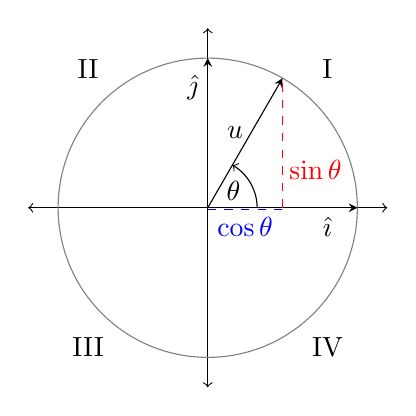
\begin{tikzpicture}[scale=1.9]
\draw [<->,black] (-1.2,0) -- (1.2,0);
\draw [<->,black] (0,-1.2) -- (0,1.2);
\draw [gray] (0,0) circle (1);
\draw[-stealth] (0,0) -- ({cos(60)}, {sin(60)});
\draw[-stealth] (0,0) -- (1, 0);
\draw[-stealth] (0,0) -- (0, 1);
\draw[-,red,dashed] ({cos(60)},0) -- ({cos(60)}, {sin(60)});
\draw[-,blue,dashed] (0,-0.01) -- ({cos(60)}, -0.01);
\draw [->,domain=0:60] plot ({0.33*cos(\x)}, {0.33*sin(\x)});
\node [right] at (0.06, 0.11) {$\theta$};
\node [below] at (0.8, 0) {$\hat{\imath}$};
\node [left] at (0, 0.8) {$\hat{\jmath}$};
\node [left] at (0.3, 0.5) {$u$};
\node [right,red] at (0.48, 0.25) {$\sin \theta$};
\node [below,blue] at (0.25, 0) {$\cos \theta$};
\node [above] at (0.8, 0.8) {I};
\node [above] at (-0.8, 0.8) {II};
\node [below] at (-0.8, -0.8) {III};
\node [below] at (0.8, -0.8) {IV};
\end{tikzpicture} 
\end{tabular}
& \ \quad  \ &
\begin{tabular}{c}
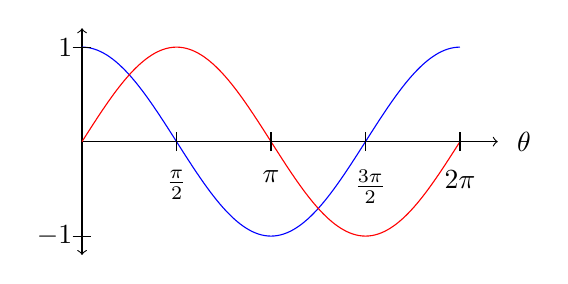
\begin{tikzpicture}[scale=1.2]
\draw [->,black] (0,0) -- (4.4,0);
\draw [<->,black] (0,-1.2) -- (0,1.2);
\draw [blue] (0,1) cos (1,0) sin (2,-1) cos (3,0) sin (4, 1);
\draw [red] (0, 0) sin (1,1) cos (2,0) sin (3,-1) cos (4,0);
\draw [-](-.1,1)--(.1,1);
\draw [-](-.1,-1)--(.1,-1);
\node [left] at (0, 1) {$1$};
\node [left] at (0, -1) {$-1$};
\draw [-](1,-0.1)--(1,0.1);
\draw [-](2,-0.1)--(2,0.1);
\draw [-](3,-0.1)--(3,0.1);
\draw [-](4,-0.1)--(4,0.1);
\node[below] at (1,-.2) {$\frac{\pi}{2}$};
\node[below] at (2,-.2) {$\pi$};
\node[below] at (3.05,-.2) {$\frac{3 \pi}{2}$};
\node[below] at (4,-.2) {$2 \pi$};
\node[right] at (4.5,0) {$\theta$};
%\matrix [draw,left] at (current bounding box.south east) {
% \node [-,blue] {$\cos \theta$}; \\
%  \node [-,red] {$\sin \theta$}; \\
%};
\end{tikzpicture}
\end{tabular}
\end{tabular}
\end{center}

We consider the angle $\theta$ between $\hat{\imath}$ and $u$. From SOH CAH TOA with H (hypotenuse) $= \|u\| = 1$, we see that $\sin \theta =$ O (opposite) and $\cos \theta =$ A (adjacent). This gives us\footnote{Note the trigonometric identity $\| u \| = \sin^2 \theta + \cos^2 \theta = 1$.}
\begin{equation*}
u = \cos \theta  \begin{bmatrix} 1 \\ 0 \end{bmatrix} + \sin \theta \begin{bmatrix} 0 \\ 1 \end{bmatrix} =  \begin{bmatrix} \cos \theta \\ \sin \theta \end{bmatrix}
\end{equation*}

We see that $\hat{\imath} \cdot u = (1, 0)^T (\cos \theta, \sin \theta) = \cos \theta$, and this relationship actually holds for any two unit vectors. Furthermore, from the plot on the right, $\cos \theta > 0$ when $| \theta | < 90\degree$ and $\cos \theta < 0$ when $| \theta | > 90\degree$.
\\

The {\bf cosine formula} further generalizes this relationship to arbitrary vectors $v$ and $w$ as follows
\begin{equation*}
\frac {v \cdot w }{\|v\| \|w\|} = \cos \theta, \qquad v \cdot w = \| v \| \| w \| \cos \theta
\end{equation*}

Thus, we have the following relationships for the dot product between any vectors $v$ and $w$:
\[
\boxed{
%\begin{eqnarray*}
\begin{aligned}
& v \cdot w > 0 & : \quad&\text{Angle between vectors is acute } (| \theta | < 90 \degree) \\
& v \cdot w = 0 & : \quad&\text{Vectors are orthogonal } (\theta = 90 \degree) \\
& v \cdot w < 0 & : \quad&\text{Angle between vectors is obtuse } (| \theta | > 90 \degree)
\end{aligned}
%\end{eqnarray*}
}
\]

Furthermore, since $| \cos \theta | \leq 1$, we see that $| v \cdot w | \leq \| v \| \| w \|$ ({\bf Cauchy-Schwartz}).
\\

From the diagram below, we also see that $\| v + w \| \leq \|v \| + \| w \|$ ({\bf Triangle Inequality}).

\begin{center}
\begin{tabular}{c c c }
\begin{tabular}{c}
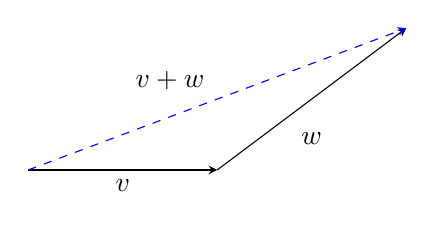
\begin{tikzpicture}[scale=1.2]
\draw [-stealth] (0,0) -- (2,0);
\draw [-stealth] (2,0) -- (4, 1.5);
\draw [-stealth,blue,dashed] (0,0) -- (4, 1.5);
\node[below] at (1,0) {$v$};
\node[below] at (3, 0.5) {$w$};
\node[above] at (1.5, 0.75) {$v+w$};
\end{tikzpicture}
\end{tabular}
& \ \quad  \ &
\begin{tabular}{c}
\begin{tikzpicture}[scale=1.2]
\draw [-stealth] (0,0) -- (1.8,0);
\draw [-stealth] (1.8,0) -- (4,0);
\draw [-stealth,blue,dashed] (0,0.5) -- (4,0.5);
\node[below] at (0.9,0) {$v$};
\node[below] at (3.1, 0) {$w$};
\node[above] at (2, 0.5) {$v+w$};
\end{tikzpicture}
\end{tabular}
\end{tabular}
\end{center}

Finally, since $v^T w = w^T v = 0$ for orthogonal vectors $v$ and $w$, we have the following:
\begin{equation*}
\| v + w \|^2 = (v + w)^T (v + w) = v^T v + v^T w + w^T v + w^T w = v^T v + w^T w  = \| v \|^2 + \| w \|^2
\end{equation*}

which is just the {\bf Pythagorean Theorem}. Similarly, we can also show $\| v - w \|^2 = \| v \|^2 + \| w \|^2$.

\subsection{Lines and Planes}

The equation for a line can be written as $x_2 = a x_1 + d$. Rearranging, we get $x_2 - a x_1 = d$. We can multiply through by an arbitrary constant and define new constants to get $c_1 x_1 + c_2 x_2 = b$. Therefore, $c^T x = b$ is the equation for a line when $c, x \in \mathbf{R}^2$. Similarly, $c^T x = b$ is the equation for a plane when $c, x \in \mathbf{R}^3$.





\section{Matrices}

We can see below that multiplying a matrix $A \in \mathbf{R}^{m \times n}$ by a vector $x \in \mathbf{R}^n$ gives a linear combination of the columns of $A$:
\begin{equation*}
A x = x_1 \begin{bmatrix} | \\ a_1 \\ | \end{bmatrix} + \dots x_n \begin{bmatrix} | \\ a_n \\ | \end{bmatrix}
\end{equation*}

Below are some definitions and rules that are often needed when manipulating matrices:
\begin{itemize}[noitemsep]
\item $AB \neq BA$ (matrix multiplication does not commute)
\item Transpose: $(AB)^T = B^T A^T$
\item Exponents: $A^p = A A \dots A$, \quad $(A^p)^q = (A^q)^p$, \quad $A^{p+q} = A^p A^q$, \quad $A^0 = I$
\end{itemize}


\subsection{Pivots and Rank}

When performing Gauss-Jordan elimination, the columns that contain the first non-zero entry for a given row are known as {\bf pivot column}s. Any column that is not a pivot column is a {\bf free column} (with an associated {\bf free variable}) and can be written as a linear combination of the pivot columns. Therefore, the number of independent columns in a matrix is the number of pivot columns.
\\

The {\bf rank} $r$ of a matrix A, $\text{rank}(A) = r$, is the number of independent columns (number of pivots\footnote{To calculate the rank of a matrix, perform Gauss-Jordan elimination and count the number of pivots.}). For any matrix $A$, the number of independent columns equals the number of independent rows, or equivalently, $\text{rank}(A) = \text{rank}(A^T)$. 
\\

We say a matrix $A \in \mathbf{R}^{m \times n}$ is {\bf full column rank} if all columns are independent ($r = n$) and {\bf full row rank} if all rows are independent ($r = m$). A square matrix is {\bf full rank} when all columns (and equivalently rows), are independent.



\subsection{Inverses}

We have the following for the {\bf inverse} of a matrix (note that $A \in \mathbf{R}^{n \times n}$ must be square):
\begin{itemize}[noitemsep]
\item Calculating the inverse of $A$: $[A | I_n] \ \rightarrow \ [I_n | A^{-1} ]$ \ (Gauss-Jordan elimination)
\item $A$ must have $n$ independent columns to be invertible (all columns have pivots): $\text{rank}(A) = n$
\item $Ax = b \ \rightarrow \ x = A^{-1} b$ \quad (the matrix is invertible if the system has a solution)
\item If $A$ is invertible, then $A x = \mathbf{0}$ has only one solution ($x$ being the zero vector).
\item If $A$ is invertible, then $\det(A) \neq 0$.
\item $A^{-1} A = I = A A^{-1}$
\item $(AB)^{-1} = B^{-1} A^{-1}$
\item $(A^{-1})^T = (A^T)^{-1}$ \quad (often writen $A^{-T}$)
\item For diagonal matrix $D$, the inverse $D^{-1}$ is also diagonal with $1/d_{ii}$ in the diagonal entries.
\item A triangular matrix is invertible iff there are no zeros on the diagonal.
\item The matrix $A^T A$ is invertible iff $A$ has independent columns.
\end{itemize}

A square matrix that is not invertible is {\bf singular}. A singular matrix $A$ has more than one solution to $A x = \mathbf{0}$ and $\det(A) = 0$.


\subsection{Determinants and Trace}

The {\bf determinant}, denoted $\det(A)$ or $|A|$, maps a square matrix $A \in \mathbf{R}^{n \times n}$ into a real number. Think of the determinant as a measure of volume: the absolute value of the determinant, $|\det(A)|$, equals the volume of the ``box" (parallelepiped) whose edges are formed by the vectors comprising the rows (or columns) of $A$. Some useful properties:

\begin{itemize}[noitemsep]
\item $\det(I) = 1$
\item Multiplying one row or column of $A$ scales $\det(A)$ by the same amount (similar to volume)
\item $\det(\alpha A) = \alpha^n \det(A)$
\item $\det(AB) = \det(A) \det(B)$
\item $\det(A) = \det(A^T)$
\item $\det(A^{-1}) = \frac{1}{\det(A)}$ \ \ (since $\det(A^{-1} A) = \det(A^{-1}) \det(A) = \det(I) = 1$)
\item $\det(A) \neq 0$ iff $\text{rank}(A) = n$ \ (i.e. if $A$ is invertible)
\item $\det(A) = 0$ iff $A$ is singular (not invertible)
\end{itemize}


The {\bf trace} of a square matrix $A \in \mathbf{R}^{n \times n}$ is defined as $\text{tr}(A) = a_{11} + \cdots + a_{nn}$ (sum of the diagonal elements of $A$). Some useful properties:
\begin{itemize}[noitemsep]
\item $\text{tr}(I) = n$
% \item $\text{tr}(\alpha A) = \alpha \det(A)$
\item $\text{tr}(A + B) = \text{tr}(A) + \text{tr}(B)$
\item $\text{tr}(A) = \text{tr}(A^T)$
\item $\text{tr}(ABC) = \text{tr}(BCA) = \text{tr}(CAB)$
\end{itemize}



\subsection{Special Matrices}

A {\bf symmetric } matrix $S \in \mathbf{R}^{n \times n}$ is any square matrix where $S^T = S$. The inverse of a symmetric matrix is also symmetric since $S^{-1} = (S^T)^{-1} = (S^{-1})^T$. Note that for \textit{any} matrix $A \in \mathbf{R}^{m \times n}$, the matrix $A^T A \in \mathbf{R}^{m \times m}$ is symmetric because $(A^T A)^T = A^T (A^T)^T = A^T A$. Similarly, $A A^T \in \mathbf{R}^{n \times n}$ is also symmetric.
\\

%Note that $u$ is a basis for the column space $C(A)$ and $v$ is a basis for the row space $C(A^T)$.

A square matrix $Q \in \mathbf{R}^{n \times n}$ is an {\bf orthogonal matrix} if it has orthonormal columns. Since $q_i^T q_j = 1$ when $i = j$ and $0$ otherwise, we have $Q^T Q = I = Q Q^T$. Therefore, $Q^T = Q^{-1}$ always holds for orthogonal matrices and the solution to $Qx = b$ is simply $x = Q^T b$ (we do not need to invert the matrix to solve the system of equations!).
\\

A {\bf rank-one matrix} is any matrix $A \in \mathbf{R}^{m \times n}$ that can be written as $A = u v^T$ (the {\bf outer product} of two vectors), where $u \in \mathbf{R}^m$ and $v \in \mathbf{R}^n$.
\\

%\item Set of all symmetric matrices: $\mathbf{S} = \{ S \in \mathbf{R}^{n \times n} | S^T = S \}$
% $A^T A \in \mathbf{S}$.

For any square matrix $A$, the {\bf matrix exponential} is defined as
\begin{equation*}
e^{At} = I + A t + \frac{1}{2} (A t)^2 + \frac{1}{6} (A t)^3 + \cdots = \sum_{k = 0}^{\infty} \frac{1}{k!} (A t)^k
\end{equation*}










\section{Vector Spaces and Subspaces}

A {\bf vector space} is a set of vectors\footnote{``Vector" can also refer to matrices or even functions (e.g. the space containing all polynomials of degree $n$).} that is {\bf closed} under scalar multiplication and vector addition.\footnote{Spaces must also obey other ``common sense" rules (e.g. $x + y = y + x$, $x + 0 = x$, $x + -x = 0$, etc).} By closed, we mean that all linear combinations of vectors in a space stay in (are contained in) the space. Note that {\it every} space contains the origin, i.e. zero vector (take the scalar multiplier $c = 0$). Vector spaces can also contain {\bf subspace}s, which are themselves spaces. Some examples:

\begin{itemize}[noitemsep]
\item The space $\mathbf{R}^n$ consists of all column vectors with $n$ components (e.g. $\mathbf{R}^2$ is the $xy$ plane). 
%\item The whole space $\mathbf{R}^n$ is a subspace.
\item The zero vector $\mathbf{0}$ is itself a subspace.
\item Lines through the origin are subspaces.
\item Planes through the origin are subspaces.
\item The quarter-plane (e.g. quadrant I) is not a subspace ($-1 v$ pushes $v$ out of the space).
\item A plane in $\mathbf{R}^3$ through the origin is a subspace of $\mathbf{R}^3$.
\item A plane in $\mathbf{R}^3$ is not in $\mathbf{R}^2$ (vectors with 3 components cannot be in $\mathbf{R}^2$).
\item $\mathbf{R}^2$ is not a subspace of $\mathbf{R}^3$ (vectors with 2 components cannot be in $\mathbf{R}^3$).
\item The set of all $x \in \mathbf{R}^n$ whose entries sum to zero (vectors with mean zero) is a subspace.\footnote{It is the nullspace of $A = (1, 1, \dots, 1)^T$, since all $x$ in the subspace satisfy $A x = \mathbf{0}$.}
\end{itemize}


The {\bf column space} (range), $C(A)$, of a matrix $A \in \mathbf{R}^{m \times n}$ consists of all linear combinations of the columns\footnote{Note that $C(A) \in \mathbf{R}^m$ (not $\mathbf{R}^n$!) because $A x$ gives a vector in $\mathbf{R}^m$, where $m$ = number of rows.} of $A$. Taking the set of all $x \in \mathbf{R}^n$, we say that $A x$ fills the column space of $A$. We can equivalently say $C(A)$ is the set of all $b$'s that satisfy $A x = b$. Note that a system $A x = b$ is only solvable if $b \in C(A)$. Some examples:
 
\begin{itemize}[noitemsep]%,topsep=0pt]
\item Any column of $A$ is in the column space of $A$ (take $x = e_i$ for any $i = 1, \dots, n$).
\item An $n \times n$ matrix has $C(A) = \mathbf{R}^n$ only when $A$ is invertible.
\item $C(A)$ is a subspace, since if $b_1, b_2 \in C(A)$, then there exist vectors $x_1$ and $x_2$ such that $A x_1 = b_1$ and $A x_2 = b_2$, and therefore, $b_1 + b_2 = A x_1 + A x_2 = A (x_1 + x_2) \in C(A)$. Furthermore, $c b_1 = c (A x_1) = A (c x_1) \in C(A)$. (linear combinations of vectors in the column space stay in the column space).
\item The solution, $x$, to $A x = b$ is not a subspace because $x = \mathbf{0}$ is not a solution (unless $b = \mathbf{0}$).
\end{itemize}

The {\bf row space} of a matrix $A$ is the column space of its transpose, $C(A^T)$.
\\

The {\bf nullspace}, $N(A)$, of a matrix $A \in \mathbf{R}^{m \times n}$ consists of all solutions\footnote{Note that $N(A) \in \mathbf{R}^n$ since $x \in \mathbf{R}^n$ for $Ax$, where $n$ = number of columns.} to $A x = \mathbf{0}$. Some examples:
\begin{itemize}[noitemsep]
\item $x = \mathbf{0}$ is always in the nullspace of any matrix $A$.
\item For an invertible matrix, $x = \mathbf{0}$ is the {\it only} solution ($N(A) = \mathbf{0}$ for $A$ invertible).
\item $N(A)$ is a subspace, since if $A x_1 = \mathbf{0}$ and $A x_2 = \mathbf{0}$, then $A(x_1 + x_2) = A x_1 + A x_2 = \mathbf{0} + \mathbf{0} = \mathbf{0}$ and $c (A x) = c  \mathbf{0} = \mathbf{0}$ (linear combinations of vectors in the nullspace stay in the nullspace).
\end{itemize}




\subsection{Independence}

The sequence of vectors $v_1, \dots, v_n$ is {\bf linearly independent} if $c_1 v_1 + \cdots + c_n v_n = \mathbf{0}$ only when $c_0, \dots, c_n$ are all zeros. Intuitively, vectors $v_1, \dots, v_n$ are independent when no vector can be written as a combination of the others. Conversely, vectors $v_1, \dots, v_n$ are {\bf linearly dependent} when at least one vector is a combination of the others.
\\

For matrices, the columns of $A$ are linearly independent when $N(A)$ contains only the zero vector (i.e. the only solution to $A x = 0$ is $x = \mathbf{0}$). This is equivalent to the matrix having full column rank\footnote{To check for independence, perform Gauss-Jordan elimination and confirm that every column has a pivot.}: $r = n$. Similarly, the columns of $A$ are dependent when there is a non-zero vector in the nullspace (i.e. rank $< n$).
\\

Some examples:
\begin{itemize}[noitemsep] %,topsep=0pt]
\item If three vectors in $\mathbf{R}^3$ are not in the same plane, they are linearly independent.
\item If three vectors in $\mathbf{R}^3$ are in the same plane, they are linearly dependent.
\item The vectors $(1, 0)$ and $(0, 1)$ are independent
\item The vectors $(1, 1)$ and $(-1, -1)$ are dependent (they lie on a line through the origin).
\item The vectors $(1, 1)$ and $(0, 0)$ are dependent (zero vector is always linearly dependent).
\item Any sequence of $n$ vectors in $\mathbf{R}^m$ will be linearly dependent for $m < n$ (i.e. the columns of any matrix with more rows than columns will be dependent).
\end{itemize}



\subsection{Span}

If we start with any set $\mathbf{S}$ of vectors in a vector space $\mathbf{V}$ (e.g. take two arbitrary vectors in $\mathbf{V} = \mathbf{R}^3$) and take all linear combinations of these vectors, we get a subspace $\mathbf{V}_s$ of $\mathbf{V}$. We say that $\mathbf{V}_s$ is {\bf spanned} by $\mathbf{S}$ (or $\mathbf{V}_s$ is the {\bf span} of $\mathbf{S}$), which means that any vector in $\mathbf{V}_s$ can be represented by a linear combination of the vectors in $\mathbf{S}$. In other words, a set of vectors {\bf spans} a space if all linear combinations of the vectors fill the space.
\\

Note that the columns of a matrix span its column space. They might be dependent.


\subsection{Orthogonality}

%We have already seen that orthogonal vectors satisfy $u^T v = 0$ and orthogonal matrices satisfy $Q^T = Q^{-1}$.
%\\

Two subspaces $V$ and $W$ of a vector space are {\bf orthogonal subspaces} if any vector $v \in V$ and any vector $w \in W$ satisfy $v^T w = 0$. We also say that $W$ is the {\bf orthogonal complement} of $V$. Some examples:
\begin{itemize}[noitemsep] %,topsep=0pt]
\item The zero vector is the only vector that is in all subspaces and is orthogonal to every subspace.
\item If the floor of a room (extended to infinity) represents a subspace and the wall of a room another subspace, they are not orthogonal because any non-vertical line drawn on the wall is not orthogonal to the line where the wall and floor meet. Furthermore, the line where the wall and floor meet is also in both subspaces, so those subspaces cannot be orthogonal.
\item The floor of a room is an orthogonal subspace to the line formed where two walls meet. In this case, the line goes through the plane at 90$\degree$.
\item The row space and nullspace of a matrix are orthogonal subspaces (orthogonal complements) in $\mathbf{R}^n$
\end{itemize}

The see the last point, note that every vector $x \in \mathbf{R}^n$ in the nullspace of $A$ is orthogonal to every row in $A$, since $( - \text{row}_i - )^T x = 0$ is always satisfied for $A x = \mathbf{0}$. Therefore, any linear combination of the dot products of each row with $x$ is also $0$, and we have that the row space and nullspace of any matrix are orthogonal. This can also be seen by noting that the row space satisfies $A^T y \subseteq \mathbf{R}^n$ for any $y \in \mathbf{R}^m$ and the nullspace satisfies $A x = \mathbf{0}$ for any $x \in \mathbf{R}^n$. Therefore, $(A^T y)^T x = y^T (A x) = y^T \mathbf{0} = 0$ and we see that the subspaces are orthogonal.




\subsection{Basis}

A {\bf basis} for a vector space is a sequence of vectors that are linearly independent and span the space. Since the basis vectors are independent, there is only one way to write a vector as a combination of the basis vectors. For a given space, the basis is not unique, but every basis has the same number of vectors. Some examples:
\begin{itemize}[noitemsep] %,topsep=0pt]
\item The $n \times n$ identity matrix $I$ is the {\bf standard basis} for $\mathbf{R}^n$.
\item The pivot columns of any $A$ are a basis for its column space.\footnote{Perform Gauss-Jordan elimination and take the original columns of $A$ corresponding to the pivot columns.}
\item The columns of {\em every} invertible matrix ($n \times n$) give a basis for $\mathbf{R}^n$. Thus, there are infinitely many bases for $\mathbf{R}^n$.
\item For any matrix $A$ with independent columns, we can construct\footnote{For instance, using the {\bf Gram-Schmidt} process, which is a generalization of projections onto lines.} a new matrix $B$ containing orthonormal columns (i.e. orthonormal basis vectors) such that $C(A) = C(B)$. 
\item Two independent vectors span a plane and are a basis for that plane. If we add one more vector in the plane, all three vectors will still span the plane, but they are not a basis because the three vectors are not independent.
\end{itemize}



\subsection{Dimension}

The {\bf dimension}  of a space is the number of basis vectors in every basis. We may think of the dimension as the ``degrees of freedom" in the space.
\\

The dimension of the column space (and row space) of a matrix $A$ is equal to $r = \text{rank}(A)$ (number of independent columns or pivots or rows). The dimension of the nullspace is equal to $n-r$ (number of free columns).


\[
\boxed{
%\begin{tabular}{r  c  l} 
%\begin{eqnarray*}
\begin{aligned}
& \quad r & = & \quad \text{rank}(A) & &\text{(Number of pivot columns)} & \\
& & = & \quad \text{dim} \ C(A) & &\text{(Number of basis vectors in the column space)} & \\
& & = & \quad \text{dim} \ C(A^T) & &\text{(Number of basis vectors in the row space)} & 
\end{aligned}
%\end{eqnarray*}
%\end{tabular}
}
\]
\
%We say the ``dimension of a space" (not ``dimension of a matrix").
%We say the ``rank of a matrix" (not ``rank of space")

Note that if you know the dimension of a space and you have $r$ independent vectors that are in the space, then those vectors form a basis for that space.









\section{Solutions of Linear Systems}


A solution, $x$, of any linear system $A x = b$ can always be expressed as the sum of:
\begin{itemize}[noitemsep]
\item A particular solution, $x_p$, satisfying $A x_p = b$. \ ($x_p$ is not necessarily unique)
\item Any vector in the nullspace, $x_n \in N(A)$, satisfying $A x_n = \mathbf{0}$. 
\end{itemize}

This is the case because $A (x_p + x_n) = A x_p + A x_n = b + \mathbf{0} = b$. Note that we are free to attach a scalar to $x_n$, since $c x_n$ stays in the nullspace, but we cannot attach a scalar to the particular solution because $A (c x_p) = c (A x_p) = c b \neq b$. 
\\

The complete solution is visualized in the figures below. If the nullspace of $A$ is 1-dimensional (i.e. there is only one free column in $A$), the nullspace takes the form of a line, as shown on the left. In this case, the particular solution shifts the nullspace away from the origin and any point on the shifted line satisfies $A x = b$. 
\begin{center}
\begin{tabular}{c c c }
\begin{tabular}{c}
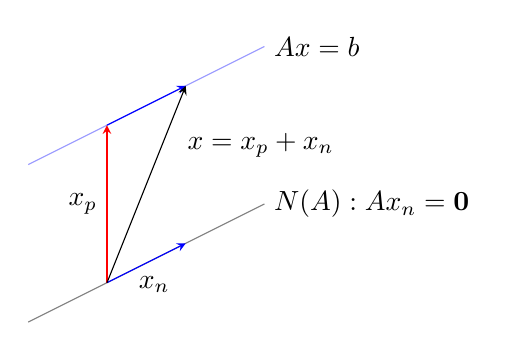
\begin{tikzpicture}[scale=1]
\draw [-,gray] (-1,-0.5) -- (2,1);
\node [right] at (2,1) {$N(A) : A x_n = \mathbf{0}$};
\draw [-,blue!50,opacity=0.8] (-1,1.5) -- (2,3);
\node [right] at (2,3) {$A x = b$};
\draw[-stealth, red] (0,0) -- (0,2);
\node [left] at (0,1) {$x_p$};
\draw[-stealth,blue] (0,2) -- (1,2.5);
\draw[-stealth,blue] (0,0) -- (1,.5);
\node [below] at (0.6,.2) {$x_n$};
\draw[-stealth] (0,0) -- (1,2.5);
\node [right] at (0.9,1.75) {$x = x_p + x_n$};
\end{tikzpicture} 
\end{tabular}
& \quad &
\begin{tabular}{c}
\tdplotsetmaincoords{110}{70}
\begin{tikzpicture}[scale=2.5,tdplot_main_coords]
\fill[blue!50,opacity=0.3] (-.5,-.5,1) -- (1.2,-.5,1) -- (1.2,1.2,1) -- (-.5,1.2,1) -- cycle;
\fill[gray!50,opacity=0.3] (-.5,-.5,0) -- (1.2,-.5,0) -- (1.2,1.2,0) -- (-.5,1.2,0) -- cycle;
\draw[-stealth,red] (0,0,0) -- (0,0,1);
\node [left] at (0.2,-.1,.5) {$x_p$};
\draw[-stealth,blue] (0,0,1) -- (.5,.5,1);
\draw[-stealth,blue] (0,0,0) -- (.5,.5,0);
\node [below] at (.2,.3,0) {$x_n$};
\draw[-stealth] (0,0,0) -- (.5,.5,1);
\node [right] at (0.25,.25,.45) {$x = x_p + x_n$};
\node[right] at (-.15,0.9,1.3) {$A x = b$};
\node[right] at (-.1,1,.3) {$N(A)$};
\end{tikzpicture}
\end{tabular}
\end{tabular}
\end{center}
When the nullspace has more than one dimension, it can be expressed as a linear combination of $n-r$ independent vectors, which fills out a (hyper) plane through the origin, as shown on the right for a two dimensional nullspace. In this case, we see that the particular solution shifts the nullspace up to the plane satisfying $A x = b$. Any value of $x$ in this plane is a solution to $Ax = b$.
\\

A special case of the complete solution is when $A$ is invertible (square, full rank). In this case, $x_n = \mathbf{0}$ (the nullspace contains only the zero vector) and the solution to $A x = b$ is just the (unique) particular solution. Furthermore, a solution always exists, since $C(A) = \mathbf{R}^n$ (all $n$-dimensional vectors are in the column space, so any $b$ can be represented as a linear combination of the columns of $A$).
\\

More generally, for a matrix $A \in \mathbf{R}^{m \times n}$, the table below shows all possibilities for solutions:
\begin{center}
\begin{tabular}{l | l | l} 
\multicolumn{1}{c|}{Rank} & \multicolumn{1}{c|}{Description} & \multicolumn{1}{c}{$Ax = b$}  \\
\hline
\hline
$r = m$ and $r = n$ & Full rank (square and invertible) & $1$ solution \\
$r = m$ and $r < n$ & Full row rank (short and wide, $m < n$, underdetermined) & $\infty$ solutions \\
$r < m$ and $r = n$ & Full column rank (tall and thin, $m > n$, overdetermined) & $0$ or $1$ solution \\
$r < m$ and $r < n$ & Not full rank & $0$ or $\infty$ solutions \\
\end{tabular}
\end{center}













\section {Projections and Least Squares}

The projection of a vector $b$ onto a line spanned by a vector $a$ is found using orthogonal vectors. From the diagram on the left, we see that error vector $e = b - p$ is orthogonal to $a$. Therefore, $a^T (b - p) = 0$, where $p = \hat{x} a$ is some multiple of $a$. Solving for $\hat{x}$, and subsequently $p$, we get
\begin{equation*}
a^T (b - \hat{x} a) = 0 \quad \rightarrow \quad \hat{x} = \frac{a^T b}{a^T a}, \qquad p = \hat{x} a = \frac{a a^T}{a^T a} b.
\end{equation*}
We call $P = (a a^T)/(a^T a)$ the {\bf projection matrix} (projector). Note that for the case of projecting onto a line, this is a rank-one matrix, since it is a column vector times a row vector (divided by a scalar). Therefore, $P$ projects onto a one-dimensional subspace (i.e. the column space of $P$ is the line through $a$). Furthermore, since $(I - P)b = b - p$, we see that $I - P$ is also a projection matrix and projects onto the line perpendicular to $a$.

\begin{center}
\begin{tabular}{c c c }
\begin{tabular}{c}
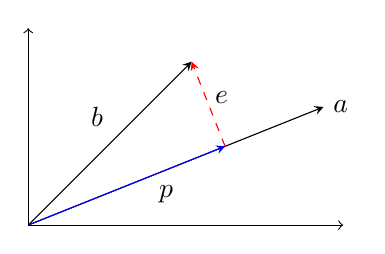
\begin{tikzpicture}[scale=2.5]
\draw [<->,black] (0,1) -- (0,0) - -(1.6,0);
\draw[-stealth] (0,0) -- (1.5,0.6);
\node [right] at (1.5,0.6) {$a$};
\draw[-stealth,blue] (0,0) -- (1,0.4);
\node [below] at (0.7,0.25) {$p$};
\draw[-stealth] (0,0) -- (0.83,0.83);
\node [above] at (0.35,0.45) {$b$};
\draw[-stealth,red,dashed] (1,0.4) -- (0.83,0.83);
\node [right] at (0.9,0.65) {$e$};
\end{tikzpicture} 
\end{tabular}
& \ \quad  \ &
\begin{tabular}{c}
\tdplotsetmaincoords{70}{20}
\begin{tikzpicture}[scale=4,tdplot_main_coords]
\fill[blue!50,opacity=0.3] (-.1,-.1,0) -- (1.1,-.1,0) -- (1.1,1.1,0) -- (-.1,1.1,0) -- cycle;
\draw[-stealth] (0,0,0) -- (.7,.7,.5);
\draw[-stealth,blue] (0,0,0) -- (.7,.7,0);
\draw[-stealth,red,dashed] (.7,.7,0) -- (.7,.7,.5);
\node[above] at (0.4,0.4,0.3) {$b$};
\node[below] at (0.4,0.4,0) {$p$};
\node[right] at (0.7,0.7,.3) {$e$};
\node[right] at (0.75,0.1,0) {$C(A)$};
\end{tikzpicture}
\end{tabular}
\end{tabular}
\end{center}

The projection of a vector $b$ onto the (hyper) plane spanned by the columns of $A$ (i.e. the column space of $A$) follows a similar approach and is illustrated in the diagram on the right. Thus, we wish to solve for $\hat{x}$ that gives us $A \hat{x} = p$, where $p$ is a vector in $C(A)$ that is closest to $b$ given the the error vector $e = b - p$. Since $e$ is orthogonal to $C(A)$, we must have\footnote{Note that since $A^T e = \mathbf{0}$, we equivalently have that vector $e$ is in the nullspace of $A^T$.} $A^T (b - A \hat{x}) = \mathbf{0}$ or $A^T A \hat{x} = A^T b$ (which is just $A x = b$ with both sides left multiplied by $A^T$). Note that $A^T A$ is square symmetric and if the columns of $A$ are independent, then $A^T A$ is invertible. This gives us the following solution and corresponding projection matrix, which projects any vector $b$ onto the column space of $A$:

\[
\boxed{
\begin{aligned}
\ A^T A \hat{x} = A^T b, \qquad \hat{x} = (A^T A)^{-1} A^T b, \qquad P = A (A^T A)^{-1} A^T \
\end{aligned}
}
\]

We also note that $P^2 = P$ since $P^2 = A (A^T A)^{-1} (A^T A) (A^T A)^{-1} A^T = A (A^T A)^{-1} A^T = P$. This is a general property of projection matrices. Intuitively, the projection of a vector that is already in the column space of $A$ does not change the vector ($p = Pb = P(Pb) = p$).
\\

If the columns of matrix $A$ are orthogonal, we have $A^T A  = I$, leading to $\hat{x} = A^T b$ and $P = A A^T$. Furthermore, if $A$ is an orthogonal matrix (square with orthonormal columns), then $\hat{x} = Q^T b$ and $P = I$. Intuitively, since the column space of $Q$ is $C(Q) = \mathbf{R}^m$, every $b$ is in $C(Q)$, and therefore the projection leaves $b$ unchanged.


\subsection{Least Squares}
The above solutions can also be derived using calculus. To start, we have the following rules for gradients (the vector of partial derivatives with respect to each vector component):
\[
\boxed{
\begin{aligned}
\ \frac{\partial}{\partial x} x^T x = 2 x, \qquad \frac{\partial}{\partial x} A x = A^T, \qquad \frac{\partial}{\partial x} x^T A x = (A + A^T) x \
\end{aligned}
}
\]

Note that for symmetric matrices, $S = S^T$, we see that the partial derivatives of $S x$ and $x^T S x$ are simply $S$ and $2 S x$, respectively.
\\

We wish to minimize the difference between $b$ and some vector in the column space of $A$ such that $\| A \hat{x} - b \|^2$ is minimized. Note that 
\begin{eqnarray*}
\| A \hat{x} - b \|^2 & = & (A \hat{x} - b)^T (A \hat{x} - b) \\
& = & \hat{x}^T A^T A \hat{x} - \hat{x}^T A^T b - b^T A \hat{x} + b^T b \\
& = & \hat{x}^T A^T A \hat{x} - 2 \hat{x}^T A^T b + b^T b
\end{eqnarray*}

where we used the fact that $\hat{x}^T A^T b \in \mathbf{R}$ is a scalar and therefore its transpose, $b^T A \hat{x}$, is equal to itself. Taking the gradient and setting it to zero, we get
\begin{equation*}
\frac{\partial}{\partial x} \left( \hat{x}^T A^T A \hat{x} - 2 \hat{x}^T A^T b + b^T b \right) = 2 A^T A \hat{x} - 2 A^T b = 0 \quad \rightarrow \quad A^T A \hat{x} = A^T b 
\end{equation*}
which is the same as the result derived using projection matrices.












\section{Eigenvectors and Eigenvalues}

Almost all vectors change direction when multiplied by a matrix, but some do not. Vectors $x$ that point in the same direction as $A x$ are {\bf eigenvector}s. Eigenvectors $x$ lie along the same line as $Ax$. We express this as $A x = \lambda x$, where $A$ is an $n \times n$ square matrix, $x$ is an eigenvector, and $\lambda$ is the {\bf eigenvalue} associated with $x$. The eigenvalue measures how much the eigenvector is stretched/shrunk when multiplied by $A$:
\begin{itemize}[noitemsep] %,topsep=0pt]
\item $|\lambda| > 1$ : $x$ is stretched by $A$
\item $|\lambda| < 1$ : $x$ is shrunk by $A$
\item $\lambda < 0$ : The direction of $x$ is reversed (but it still remains on the same line as $x$).
\item $\lambda = 0$ : $x$ is in the nullspace\footnote{This is still considered to be on the line as $x$, since every vector passes through the origin.} of $A$
\end{itemize}

Since $A x = \lambda x$ can be rewritten as $(A - \lambda I) x = 0$, we see that eigenvectors make up the nullspace of the matrix $(A - \lambda I)$. Furthermore, if there is a nonzero solution, then $(A - \lambda I)$ is not invertible (i.e. it is singular) and therefore $\det (A - \lambda I) = 0$. Writing out the determinant gives us the {\bf characteristic equation} (polynomial of degree $n$) and solving for the roots gives us the eigenvalues. Note that there are $n$ roots (eigenvalues) for an $n \times n$ matrix.\footnote{But multiple eigenvalues can have the same value. Eigenvalues can also be complex (conjugates) even if $A$ is real.} For each eigenvalue, $\lambda_i$, the matrix $(A - \lambda_i I)$ is singular (there is a nonzero $x_i$ in the nullspace), so we can solve for $x_i$ that gives $(A - \lambda_i I) x_i = 0$. These $x_i$ are the eigenvectors.
\\

For example, for a $2 \times 2$ matrix, we have\footnote{Note that this is equal to $\lambda^2 - \text{tr}(A) \lambda + \det(A)$}
\begin{equation*}
\det (A -\lambda I) = \begin{vmatrix} a - \lambda & b \\ c & d - \lambda \end{vmatrix} = (a - \lambda) (d - \lambda) - b c = \lambda^2 - a d \lambda + (a d - b c) = 0
\end{equation*}

Solving for the roots of this characteristic polynomial gives us the two eigenvalues $\lambda_1$ and $\lambda_2$. Plugging each $\lambda_i$ into $(A - \lambda_i I) x_i = 0$ and solving each system of equations gives us two eigenvectors $x_1$ and $x_2$.
\\

Note that eigenvectors are not unique. If we multiply both sides of $A x = \lambda x$ by a scalar $c$, we get $c (A x) = c (\lambda x) \rightarrow A(cx) = \lambda (cx)$, so $cx$ is also a valid eigenvector, albeit one that still lies on the same line as $x$. Eigenvectors are commonly scaled so that they are all unit vectors.
\\

Some useful properties of eigenvalues and eigenvectors:
\begin{itemize}[noitemsep] %,topsep=0pt]
\item $\text{tr}(A) = \lambda_1 + \cdots + \lambda_n$ \quad  (the sum of the eigenvalues equals the trace)
\item $\det (A) = \lambda_1 \cdots \lambda_n$ \ \qquad (the product of the eigenvalues equals the determinant)
\item The diagonal entries of a triangular matrix are its eigenvalues.
\item $(c A) x = (c \lambda) x$ \quad (scaling a matrix leaves the eigenvectors alone but scales the eigenvalues)
\item $A^k x = \lambda^k x$ \qquad \ \ (e.g. for $k = 2$, we have  $A^2 x= A A x = A (\lambda x) = \lambda^2 x$)
\item If $A$ is singular (not invertible), at least one $\lambda = 0$ (other $\lambda$'s can be nonzero)
\item If $A$ is invertible, $\lambda = 0$ cannot be an eigenvalue (we shift $A$ by $\lambda$ to make it singular)
\item $A^{-1} x = \lambda^{-1} x$ \ \ (the eigenvalues of the inverse of a matrix are the inverses of the eigenvalues)
%\item $(A + cI) x = (\lambda + c) x$ since $(A + cI) x  = A x + c (I x) = \lambda x + c x = (\lambda + c) x$
\end{itemize}







% Any vector can be expressed as a linear combination of the eigenvectors. 


%A zero eigenvealue means $A x = 0 x = 0$, which means the eigenvector is in the nullspace of $A$.

Most matrices $A \in \mathbf{R}^{n \times n}$ have $n$ eigenvector directions and $n$ distinct eigenvalues, but some types of matrices have unique properties:
\begin{itemize}[noitemsep] %,topsep=0pt]
\item Symmetric matrices have orthogonal eigenvectors (which can be scaled to be orthonormal)
\item Identity matrices ($Ix = x$): All vectors are eigenvectors of $I$ and all $\lambda$'s are $1$
\item Projection matrices: 
\begin{itemize}[noitemsep,topsep=0pt,label=$\circ$]
\item If $x$ is in the column space, then $Px = x$ and $\lambda = 1$ (the column space projects onto itself, so projection does not change $x$).
\item If $x$ is orthogonal to the column space, then $Px = 0$ and $\lambda = 0$ ($x$ is in the null space).
\item Projection matrices (and only projection matrices) only have eigenvalues that are either $0$ or $1$.
\end{itemize}
\end{itemize}



%\subsection{Dynamical Systems}

% Differential equations $\frac{du}{dt} = Au$.

%$\lambda < 1$ (decay), $\lambda = 1$ (steady state), $\lambda > 1$.

%When $| \lambda | < 1 \ \forall \ \lambda$, then $A^k \rightarrow \infty$.


\subsection{Diagonalizing a Matrix}

We may write $Ax_i = \lambda_i x_i$ in matrix form by placing the all eigenvectors into the columns of a matrix $X$ and all the the eigenvalues into a diagonal marix $\Lambda$ as follows
\begin{equation*}
A X = A  \begin{bmatrix} | & & | \\ x_1 & \hspace{-1em} \cdots \hspace{-1em}  & x_n \\ | & & | \end{bmatrix} = \begin{bmatrix} | & & | \\ x_1 & \hspace{-1em} \cdots \hspace{-1em}  & x_n \\ | & & | \end{bmatrix} \begin{bmatrix} \vspace{-0.3em} \lambda_1 & &  \\  & \hspace{-1em} \ddots \hspace{-1em} &  \\  & & \lambda_n \end{bmatrix} = X \Lambda
\end{equation*}

where we refer to $X$ as the eigenvector matrix and $\Lambda$ as the eigenvalue matrix.
\\

If all the eigenvalues in $\Lambda$ are different, then all eigenvectors are guaranteed to be independent. If there are repeated eigenvalues, then we must check the eigenvectors to see if they are independent.\footnote{For instance, the identity matrix has all $\lambda_i = 1$, but the eigenvectors are independent ($X$ can be {\em any} basis in $\mathbf{R}^n$ for \\ $\text{ \quad \ \ }$ the identity matrix).}
\\

If a real matrix $A \in \mathbf{R}^{n \times n}$ has linearly independent eigenvectors $x_1, \cdots, x_n$, then the eigenvector matrix $X$ is invertible and we say that $A$ is {\bf diagonalizable}.\footnote{If the eigenvectors are not all independent, then matrix $A$ is not diagonalizable.} Diagonalizable matrices can therefore be written as $A = X \Lambda X^{-1}$ or alternatively $\Lambda = X^{-1} A X$.
\\

Note that since $A^2 = AA = (X \Lambda X^{-1}) (X \Lambda X^{-1}) = X \Lambda (X^{-1} X) \Lambda X^{-1} = X \Lambda^2 X^{-1}$, squaring a matrix squares the eigenvalues but leaves the eigenvectors unchanged. More generally, $A^k = X \Lambda^k X^{-1}$.
\\

Similarly, for any diagonalizable matrix $A$, we have
\begin{equation*}
e^{At} = \sum_{k = 0}^{\infty} \frac{1}{k!} (A t)^k = \sum_{k = 0}^{\infty} \frac{1}{k!} X (\Lambda t)^k X^{-1} = X \left( \sum_{k = 0}^{\infty} \frac{1}{k!} (\Lambda t)^k \right) X^{-1} = X e^{\Lambda t} X^{-1}
\end{equation*}



\subsection{Symmetric and Positive Definite Matrices}

Symmetric matrices have only {\em real} eigenvalues and {\em orthogonal} eigenvectors, which can be normalized to be {\em orthonormal}. The {\bf spectral theorem} (principal axis theorem) says that every symmetric matrix has factorization $S = Q \Lambda Q^T$, where the eigenvector matrix ($X = Q$) is orthogonal ($Q^{-1} = Q^T$).\footnote{Note that $Q \Lambda Q^T$ is symmetric since $(Q \Lambda Q^T)^T = (Q^T)^T \Lambda^T Q = Q \Lambda Q^T$.} Expanding out the factorization, we have\footnote{Try this with $2 \times 2$ matrices for $Q$ and $\Lambda$ to convince yourself it holds.}:
\begin{eqnarray*}
S & = & Q \Lambda Q^T =  \begin{bmatrix} | & & | \\ x_1 & \hspace{-2em} \cdots \hspace{-2em}  & x_n \\ | & & | \end{bmatrix} \begin{bmatrix} \vspace{-0.3em} \lambda_1 & &  \\  & \hspace{-1em} \ddots \hspace{-1em} &  \\  & & \lambda_n \end{bmatrix} \begin{bmatrix} \text{---} \hspace{-1em} & x_1 & \hspace{-1em} \text{---} \\ & \vspace{-0.2em} \vdots  \vspace{-0.2em} & \\ \text{---} \hspace{-1em} & x_n & \hspace{-1em} \text{---} \end{bmatrix} = \begin{bmatrix} | & & | \\ \lambda_1 x_1 & \hspace{-2em} \cdots \hspace{-2em}  & \lambda_n x_n \\ | & & | \end{bmatrix} \begin{bmatrix} \text{---} \hspace{-1em} & x_1 & \hspace{-1em} \text{---} \\ & \vspace{-0.2em} \vdots  \vspace{-0.2em} & \\ \text{---} \hspace{-1em} & x_n & \hspace{-1em} \text{---} \end{bmatrix} \\
& = & \lambda_1 x_1 x_1^T + \cdots + \lambda_n x_n x_n^T = \lambda_1 P_1 + \cdots + \lambda_n P_n
\end{eqnarray*}

where $P_i = x_i x_i^T$ are rank-one projection matrices, and we see that a symmetric matrix $A$ can be written as a linear combination of projection matrices weighted by their eigenvalues.
\\

%Symmetric $A$ can be written as a sum of rank-one matrices


%The nullspace is perpendicular to the column space for a symmetric matrix.

A symmetric matrix with all {\em positive} real eigenvalues is a {\bf positive definite} matrix. Equivalently, a matrix $A$ is positive definite if $x^T A x > 0$ for every non-zero vector $x$.\footnote{A matrix is also positive definite if all principal minors (upper left determinants) are positive:\\ $\text{ \quad \ \ } a_{11} > 0, a_{11} a_{22} - a_{21} a_{12} > 0, \cdots, \det(A) > 0$} If the eigenvalues are non-negative (i.e. $\lambda_i \geq 0$), the matrix is {\bf positive semidefinite} and $x^T A x \geq 0$.
\\


%For $2 \times 2$ matrix, the eigenvalues of $A = \begin{bmatrix} a & b \\ b & c \end{bmatrix}$ are positive iff $a > 0$ and $ac - b^2 > 0$ (positive principal minors, e.g. upper left determinants).

If $A$ and $B$ are positive (semi) definite, so is $A+B$ because $x^T (A + B) x = x^T A x + x^T B x > 0$.
\\

For any matrix $R$ with independent columns, the symmetric matrix $A = R^T R$ is positive definite since $x^T A x = x^T R^T Rx = (Rx)^T (Rx) = \| Rx \|^2 > 0$ (because square of real number is positive).
\\

It can also be shown that every positive definite matrix $A$ can be written as $A = L L^T$, where $L$ is lower triangular ({\bf Cholesky decomposition}).
\\

%\item $Rx \neq 0$ when $x \neq 0$ because columns are independent

%When a symmetric matrix has one of the following properites, it has them all:
%\begin{itemize}[noitemsep] %,topsep=0pt]
%\item All $n$ eigenvalues are positive
%\item $x^T A x > 0$ except at $x = 0$
%\item $A = R^T R$ for a matrix $R$ with independent columns (Cholesky)
%\item All $n$ leading principal minors (upper left determinants) are positive: \\ $a_{11} > 0, a_{11} a_{22} - a_{21} a_{12} > 0, \cdots, \det(A) > 0$
%\end{itemize}


%\subsection{Singular Value Decomposition (SVD)}


%\subsection{Principal Components Analysis}




















\

\

\begin{thebibliography}{9}

\bibitem{BV} Boyd, S. and L. Vandenberghe (2004). \textit{\href{https://web.stanford.edu/~boyd/cvxbook/}{Convex Optimization}}, Cambridge University Press.

\bibitem {ESL} Hastie, T., R. Tibshirani, and J. Friedman (2009). \textit{\href{https://web.stanford.edu/~hastie/ElemStatLearn/}{The Elements of Statistical Learning: Data Mining, Inference, and Prediction.}}, 2nd Ed., Springer.

\bibitem {Murphy} Murphy, K. P. (2012). \textit{\href{https://probml.github.io/pml-book/book0.html}{Machine Learning: A Probabilistic Perspective}}, MIT Press.

\bibitem {Strang1} Strang, G. (2005). MIT 18.06 Linear Algebra [Video lectures]. YouTube. \\
\href{https://www.youtube.com/playlist?list=PLE7DDD91010BC51F8}{https://www.youtube.com/playlist?list=PLE7DDD91010BC51F8}

\bibitem{Strang2} Strang, G. (2016). \textit{Introduction to Linear Algebra}, 5th Ed., Wellesley-Cambridge Press.

\end{thebibliography}





\end{document}